\documentclass[a4paper, UTF8]{ctexart}
\usepackage{ctex}
\usepackage{amsmath}
\usepackage{amsthm}
\usepackage{multirow}
\usepackage{amssymb}
\usepackage{graphicx}
\usepackage{geometry}
\usepackage{bm}
\usepackage{subfigure}
\usepackage{float}
\usepackage{mathrsfs}
\renewcommand\thesection{\arabic{section}}
\newtheorem*{exercise}{\textbf{习题}}
\newtheorem*{theorem}{Theorem}
\title{Manifole Learning Homework 4}
\date{\today}
\author{安捷 1601210097}
\begin{document}
\maketitle
  \begin{exercise}[50]
    \begin{proof}
      已知目标函数为
      \begin{equation}
        \frac{1}{2} \sum_{i,j=1}^k \pi_i p_{ij}\left( \frac{g_i}{\sqrt{\pi_i}} - \frac{g_j}{\sqrt{\pi_j}}\right)^2,\quad s.t.\quad \lVert \mathbf{g} \rVert = 1
      \end{equation}
      \begin{equation}
        = \frac{1}{2}\sum_{i,j=1}^k \pi_i p_{ij} \frac{g_i^2}{\pi_i} + \frac{1}{2}\sum_{i,j=1}^k\pi_i p_{ij} \frac{g_j^2}{\pi_j} + \frac{1}{2} \sum_{i,j=1}^k \pi_i p_{ij}\frac{g_i g_j}{\sqrt{\pi_i} \sqrt{\pi_j}} + \frac{1}{2} \sum_{i,j=1}^k \pi_i p_{ij}\frac{g_j g_i}{\sqrt{\pi_j} \sqrt{\pi_i}}
      \end{equation}
      由于
      \begin{equation}
        \sum_{j=1}^kp_{ij} = 1, \qquad \sum_{i = 1}^k \pi_i p_{ij} = \pi_j
      \end{equation}
      所以有
      \begin{equation}
        \frac{1}{2}\sum_{i,j=1}^k \pi_i p_{ij}\frac{g_i^2}{\pi_i} = \frac{1}{2}\sum_{i,j=1}^k \pi_i p_{ij}\frac{g_j^2}{\pi_j} = \frac{1}{2}\sum_{i=1}^k g_i^2 = \mathbf{g}^T \mathbf{I} \mathbf{g}
      \end{equation}
      而剩余两项可以写为
      \begin{equation}
        \frac{1}{2} \sum_{i,j=1}^k \pi_i p_{ij}\frac{g_i g_j}{\sqrt{\pi_i} \sqrt{\pi_j}} + \frac{1}{2} \sum_{i,j=1}^k \pi_i p_{ij}\frac{g_j g_i}{\sqrt{\pi_j} \sqrt{\pi_i}}
      \end{equation}
      \begin{equation}
        = \frac{1}{2} \sum_{i,j=1}^k \sqrt{\pi_i} p_{ij}\frac{g_i g_j}{\sqrt{\pi_j}}+ \frac{1}{2} \sum_{i,j=1}^k \sqrt{\pi_j} p_{ji}\frac{g_i g_j}{\sqrt{\pi_i}}
      \end{equation}
      \begin{equation}
        = \frac{1}{2}\mathbf{g}^T\left( \Pi^{\frac{1}{2}}\mathbf{P}\Pi^{-\frac{1}{2}} + \Pi^{-\frac{1}{2}} \mathbf{P}^T \Pi^{\frac{1}{2}} \right)\mathbf{g} = \Theta
      \end{equation}
      其中
      \begin{equation}
        \Pi = \mathrm{diag}\left( \pi \right)
      \end{equation}
      所以原式可以写成矩阵形式
      \begin{equation}
        \mathbf{g}^T \left( \mathbf{I} - \Theta \right) \mathbf{g}. \quad s.t. \quad \lVert \mathbf{g}\rVert = 1
      \end{equation}
    \end{proof}
  \end{exercise}
  \begin{exercise}[51]
    在这个问题中我选择了UMIST数据集中的前两个人脸数据,分类准确率=\rm{0.5479},我认为具有较低准确率的原因在于,欧式距离不能很好的度量两个人脸的相似性,因为不同视角的人脸的欧式距离很大,因此,使用更为合适的距离度量或许可以显著提高分类的准确率。
  \end{exercise}
  \begin{exercise}[57]
    \rm{PCA} 与标准化 \rm{PCA} 求得的平均脸如下图所示:
    \begin{figure}[htbp!]
      \centering
      \subfigure[PCA mean face]{
      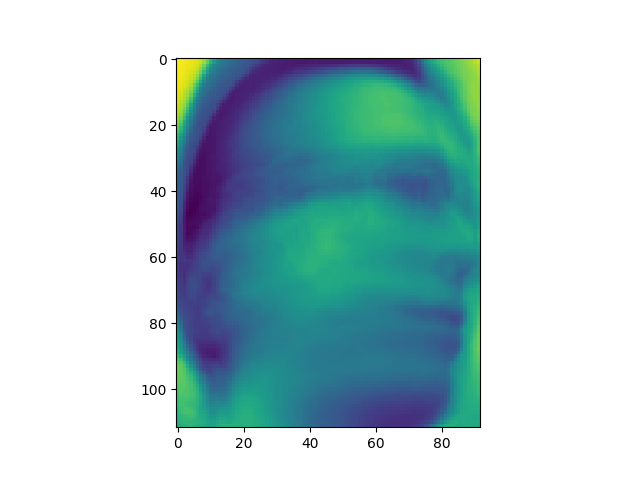
\includegraphics[width=0.45\textwidth]{fig57_1.png}
      }
      \subfigure[scaled PCA mean face]{
      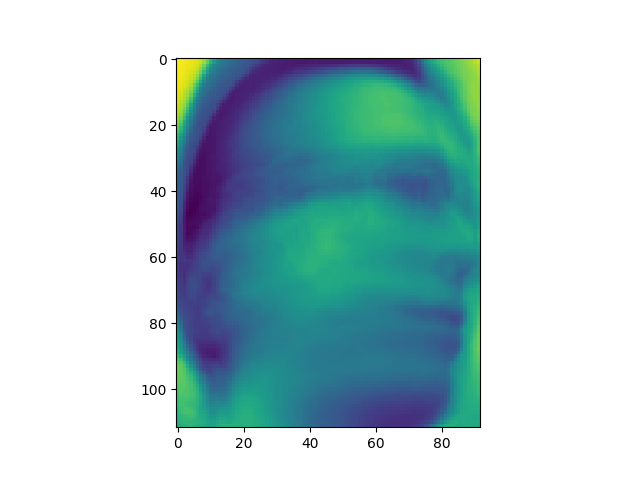
\includegraphics[width=0.45\textwidth]{fig57_2.png}
      }
      \caption{mean face result}
    \end{figure}
  \end{exercise}
\end{document}
